\documentclass[a4paper, titlepage, 12pt]{article}
\usepackage{graphicx}
\usepackage{color}
\usepackage{hyperref}
\usepackage{amsmath}
\usepackage{amsthm}
\usepackage{adjustbox}
\usepackage{float}
\usepackage{mdframed}
\usepackage{subfig}
\DeclareMathOperator{\argmax}{arg\,max}
\numberwithin{equation}{section}
% For box
\usepackage{collectbox}

\makeatletter
\newcommand{\mybox}{%
    \collectbox{%
        \setlength{\fboxsep}{1pt}%
        \fbox{\BOXCONTENT}%
    }%
}
\makeatother
%Endfor box



\begin{document}
    \title{ECE - 5534 Electronic Design Automation \\ ROBDDs}
    \author{Prathamesh Mandke \\ \href{pkmandke@vt.edu}{pkmandke@vt.edu} \\ PID: 906239574}
    \date{\today \\ \href{https://ece.vt.edu}{ECE} @ \href{https://vt.edu}{Virginia Tech}}
    \maketitle
    \newpage

    \section{Lab Overview}

        Reduced Ordered Binary Decision Diagrams (ROBDDs) are concise representations of boolean expressions in the form of a directed acyclic graph.
        ROBDDs make use of the if-then-else (INF) form of boolean expressions to construct the graphical representation.
        An INF form of a boolean expression is one where any operations are only perfomed on variables with constants and INF statements.
        The practicality of using the INF form to construct ROBDDs for any boolean expression stems from the Shannon Expansion idea.
        Shannon Expansion involves breaking down an expression (with arbitrary number of variables) into an INF form by recursively setting and resetting the value of one variable at a time.
        From the perspective of implementation in digital logic, the Shannon Expansion involves cascading multiplexer circuits by considering all combinations of a boolean variable at a time.
        
        When a complicated boolean expression is recursively broken down into it's INF, a series of INF statements are obtained.
        Now, if any redundant INF statements are combined, the resulting set of INF statements can be expressed as a binary decision diagram.
        When the order of variable selection is same across all recursive builds of the INF forms, the resulting decision diagram has nodes in the same order starting from the root.
        Such a BDD is said to be an ordered BDD.
        Going one step further, multiple nodes with the same left and right nodes can be combined since they are obviously redundant.
        Such reduction leads to a unique representation of the boolean expression known as the ROBDD.
        However, it is interesting to note that this representation is not unique to the order of variable selection and is in fact highly sensitive to it.
        
        This work involves the implementation of a ROBDD for boolean operations AND, OR, NOT, IMPLICATION and EQUIVALENCE.
        The methods used to implement the ROBDD have been inspired from Henrik Anderson's document on Binary Decision Diagrams.

    \section{Tests}

        This section involves multiple tests and their results for verifying the functionality.
        Initially, I have considered simple unit tests for verifying the correctness of individual methods such as Build, Apply, etc. 
        Further, there are somewhat non-trivial and nuanced test cases for demonstrating the usefulness, simplicity and effectiveness of ROBDDs.

        \subsection{Unit Tests}

            This section includes unit tests for verifying functionality of individual methods of the ROBDD implementation.

            \begin{itemize}
                \item[1.] \textbf{Build (and Make)}
                    
                    It was difficult to find online utilities that could generate the T table for a given expression.
                    Thus, I have attempted to verify the same example as in the Henrik Anderson's document.
                    The expression in the document is "and(equiv(x1, x2), equiv(x2, x3))".

                    \begin{figure}[htp]
                        \centering
                        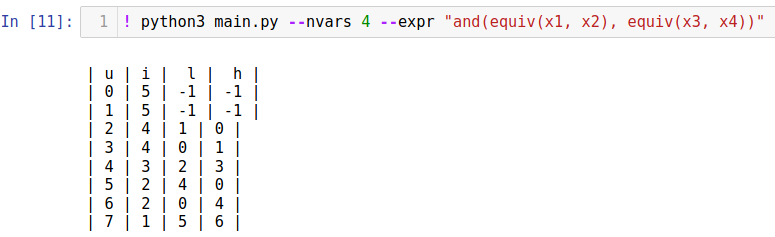
\includegraphics[height=0.3\textwidth, width=\textwidth]{img/robdd_build.png}
                        \caption{Program output}
                        \label{fig:build_prog_out}
                    \end{figure}
                    
                    \begin{figure}[htp]
                        \centering
                        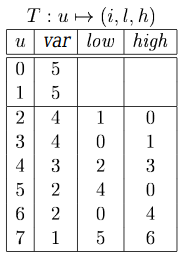
\includegraphics[height=140px, width=180px]{img/true_T_build.png}
                        \caption{True output}
                        \label{fig:build_true_out}
                    \end{figure}

                    The fact that the resulting BDD is also in the reduced form verifies the functionality of the Make (Mk) function as well.
                \item[2.] \textbf{Apply}
                    
                    Consider Figure \ref{fig:test_apply}.

                    \begin{figure}[htp]
                        \centering
                        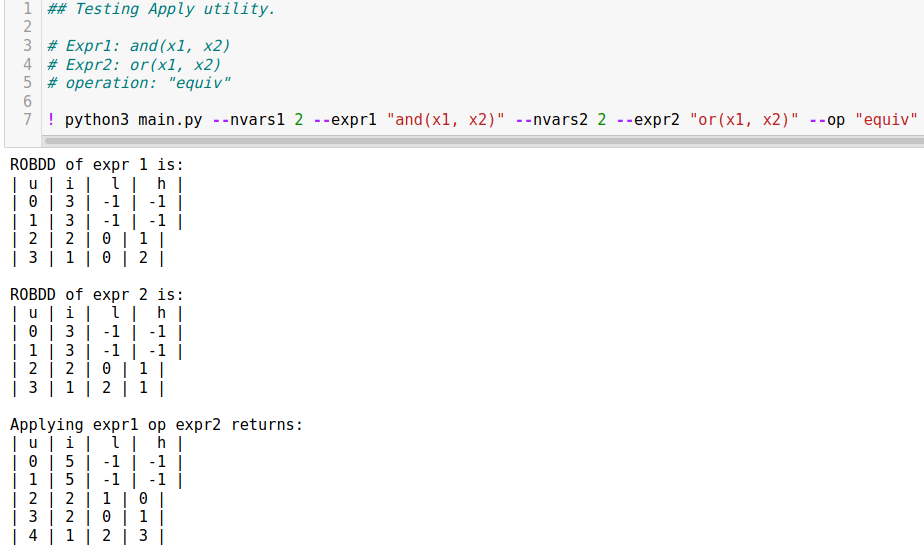
\includegraphics[height=200px, width=400px]{img/test_apply.png}
                        \caption{Testing Apply utility.}
                        \label{fig:test_apply}
                    \end{figure}

                    It is easy to observe that for the resulting expression "equiv(and(x1, x2), or(x1, x2))" the T table is correct.
                    Starting from the root node number 4, if $x1 = 0$ we check node 2 and if $x1 = 1$ we check node 3.
                    Now, if $x1 = 0$ then $and(x1, x2) = 0$ and the equivalence will only be true if $or(x1, x2)$ is true, that is, if $x2 = 1$.
                    This is verified from row number 3 of the resulting T table obtained after applying the equiv operation.
                    Similarly, the behaviour for $x1 = 1$ can be verified easily.

                \item[3.] \textbf{Restrict}

                    To verify that restrict works as intended, consider the expression or(and(x1, x2), x2).
                    Figure \ref{fig:test_restrict}, contains the results for all 4 settings of the 2 variables $x1$ and $x2$.

                    \begin{figure}[htp]
                        \centering
                        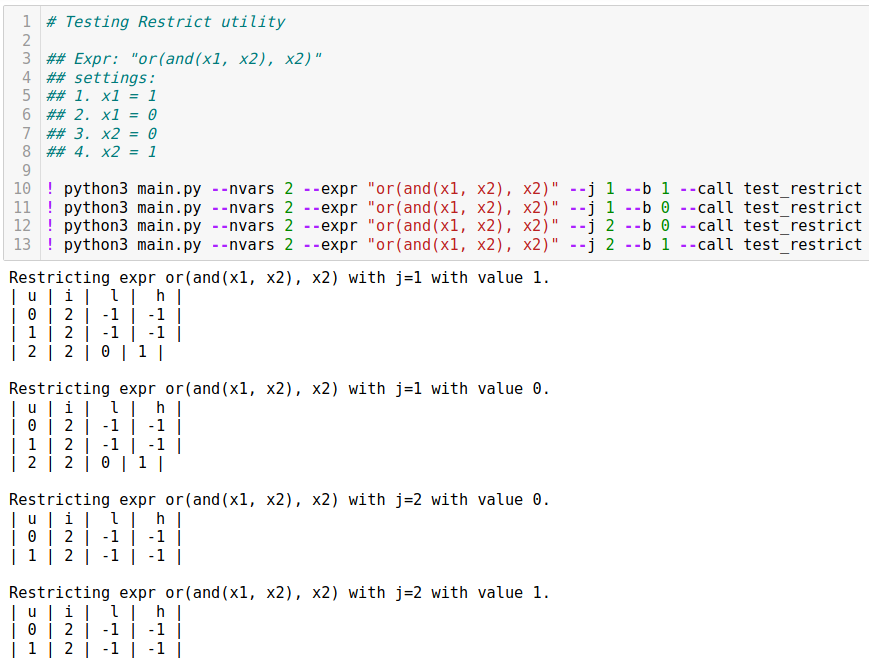
\includegraphics[height=250px, width=350px]{img/test_restrict.png}
                        \caption{Testing Restrict utility.}
                        \label{fig:test_restrict}
                    \end{figure}

                    It can be observed that when $x1 = 0$, the expression is 0 if x2 is 0 else it is 1.
                    Moreover, if $x1 = 1$, the expression is 0 if x2 is 0 else it is 1.
                    With $x2 = 0$, the expression will always be 0 while if $x2 = 1$ the expression is a tautology.
                    In the last 2 cases, the root of the ROBDD changes although the T table looks alike.

                \item[4.] \textbf{StatCount, AnySat and AllSat}
                
                    Until now, I have considered relatively trivial examples since it was difficult to obtain T tables to compare and verify correctness.
                    However, for the statistical measures, the University of Utah provides a BDD interface for result verification at this URL [1].

                    Consider the expression 

            \end{itemize}
    
    \section{References}

            [1]  \href{http://formal.cs.utah.edu:8080/pbl/BDD.php}{http://formal.cs.utah.edu:8080/pbl/BDD.php}
\end{document}